\documentclass[1p]{elsarticle_modified}
%\bibliographystyle{elsarticle-num}

%\usepackage[colorlinks]{hyperref}
%\usepackage{abbrmath_seonhwa} %\Abb, \Ascr, \Acal ,\Abf, \Afrak
\usepackage{amsfonts}
\usepackage{amssymb}
\usepackage{amsmath}
\usepackage{amsthm}
\usepackage{scalefnt}
\usepackage{amsbsy}
\usepackage{kotex}
\usepackage{caption}
\usepackage{subfig}
\usepackage{color}
\usepackage{graphicx}
\usepackage{xcolor} %% white, black, red, green, blue, cyan, magenta, yellow
\usepackage{float}
\usepackage{setspace}
\usepackage{hyperref}

\usepackage{tikz}
\usetikzlibrary{arrows}

\usepackage{multirow}
\usepackage{array} % fixed length table
\usepackage{hhline}

%%%%%%%%%%%%%%%%%%%%%
\makeatletter
\renewcommand*\env@matrix[1][\arraystretch]{%
	\edef\arraystretch{#1}%
	\hskip -\arraycolsep
	\let\@ifnextchar\new@ifnextchar
	\array{*\c@MaxMatrixCols c}}
\makeatother %https://tex.stackexchange.com/questions/14071/how-can-i-increase-the-line-spacing-in-a-matrix
%%%%%%%%%%%%%%%

\usepackage[normalem]{ulem}

\newcommand{\msout}[1]{\ifmmode\text{\sout{\ensuremath{#1}}}\else\sout{#1}\fi}
%SOURCE: \msout is \stkout macro in https://tex.stackexchange.com/questions/20609/strikeout-in-math-mode

\newcommand{\cancel}[1]{
	\ifmmode
	{\color{red}\msout{#1}}
	\else
	{\color{red}\sout{#1}}
	\fi
}

\newcommand{\add}[1]{
	{\color{blue}\uwave{#1}}
}

\newcommand{\replace}[2]{
	\ifmmode
	{\color{red}\msout{#1}}{\color{blue}\uwave{#2}}
	\else
	{\color{red}\sout{#1}}{\color{blue}\uwave{#2}}
	\fi
}

\newcommand{\Sol}{\mathcal{S}} %segment
\newcommand{\D}{D} %diagram
\newcommand{\A}{\mathcal{A}} %arc


%%%%%%%%%%%%%%%%%%%%%%%%%%%%%5 test

\def\sl{\operatorname{\textup{SL}}(2,\Cbb)}
\def\psl{\operatorname{\textup{PSL}}(2,\Cbb)}
\def\quan{\mkern 1mu \triangleright \mkern 1mu}

\theoremstyle{definition}
\newtheorem{thm}{Theorem}[section]
\newtheorem{prop}[thm]{Proposition}
\newtheorem{lem}[thm]{Lemma}
\newtheorem{ques}[thm]{Question}
\newtheorem{cor}[thm]{Corollary}
\newtheorem{defn}[thm]{Definition}
\newtheorem{exam}[thm]{Example}
\newtheorem{rmk}[thm]{Remark}
\newtheorem{alg}[thm]{Algorithm}

\newcommand{\I}{\sqrt{-1}}
\begin{document}

%\begin{frontmatter}
%
%\title{Boundary parabolic representations of knots up to 8 crossings}
%
%%% Group authors per affiliation:
%\author{Yunhi Cho} 
%\address{Department of Mathematics, University of Seoul, Seoul, Korea}
%\ead{yhcho@uos.ac.kr}
%
%
%\author{Seonhwa Kim} %\fnref{s_kim}}
%\address{Center for Geometry and Physics, Institute for Basic Science, Pohang, 37673, Korea}
%\ead{ryeona17@ibs.re.kr}
%
%\author{Hyuk Kim}
%\address{Department of Mathematical Sciences, Seoul National University, Seoul 08826, Korea}
%\ead{hyukkim@snu.ac.kr}
%
%\author{Seokbeom Yoon}
%\address{Department of Mathematical Sciences, Seoul National University, Seoul, 08826,  Korea}
%\ead{sbyoon15@snu.ac.kr}
%
%\begin{abstract}
%We find all boundary parabolic representation of knots up to 8 crossings.
%
%\end{abstract}
%\begin{keyword}
%    \MSC[2010] 57M25 
%\end{keyword}
%
%\end{frontmatter}

%\linenumbers
%\tableofcontents
%
\newcommand\colored[1]{\textcolor{white}{\rule[-0.35ex]{0.8em}{1.4ex}}\kern-0.8em\color{red} #1}%
%\newcommand\colored[1]{\textcolor{white}{ #1}\kern-2.17ex	\textcolor{white}{ #1}\kern-1.81ex	\textcolor{white}{ #1}\kern-2.15ex\color{red}#1	}

{\Large $\underline{10_{87}~(K10a_{39})}$}

\setlength{\tabcolsep}{10pt}
\renewcommand{\arraystretch}{1.6}
\vspace{1cm}\begin{tabular}{m{100pt}>{\centering\arraybackslash}m{274pt}}
\multirow{5}{120pt}{
	\centering
	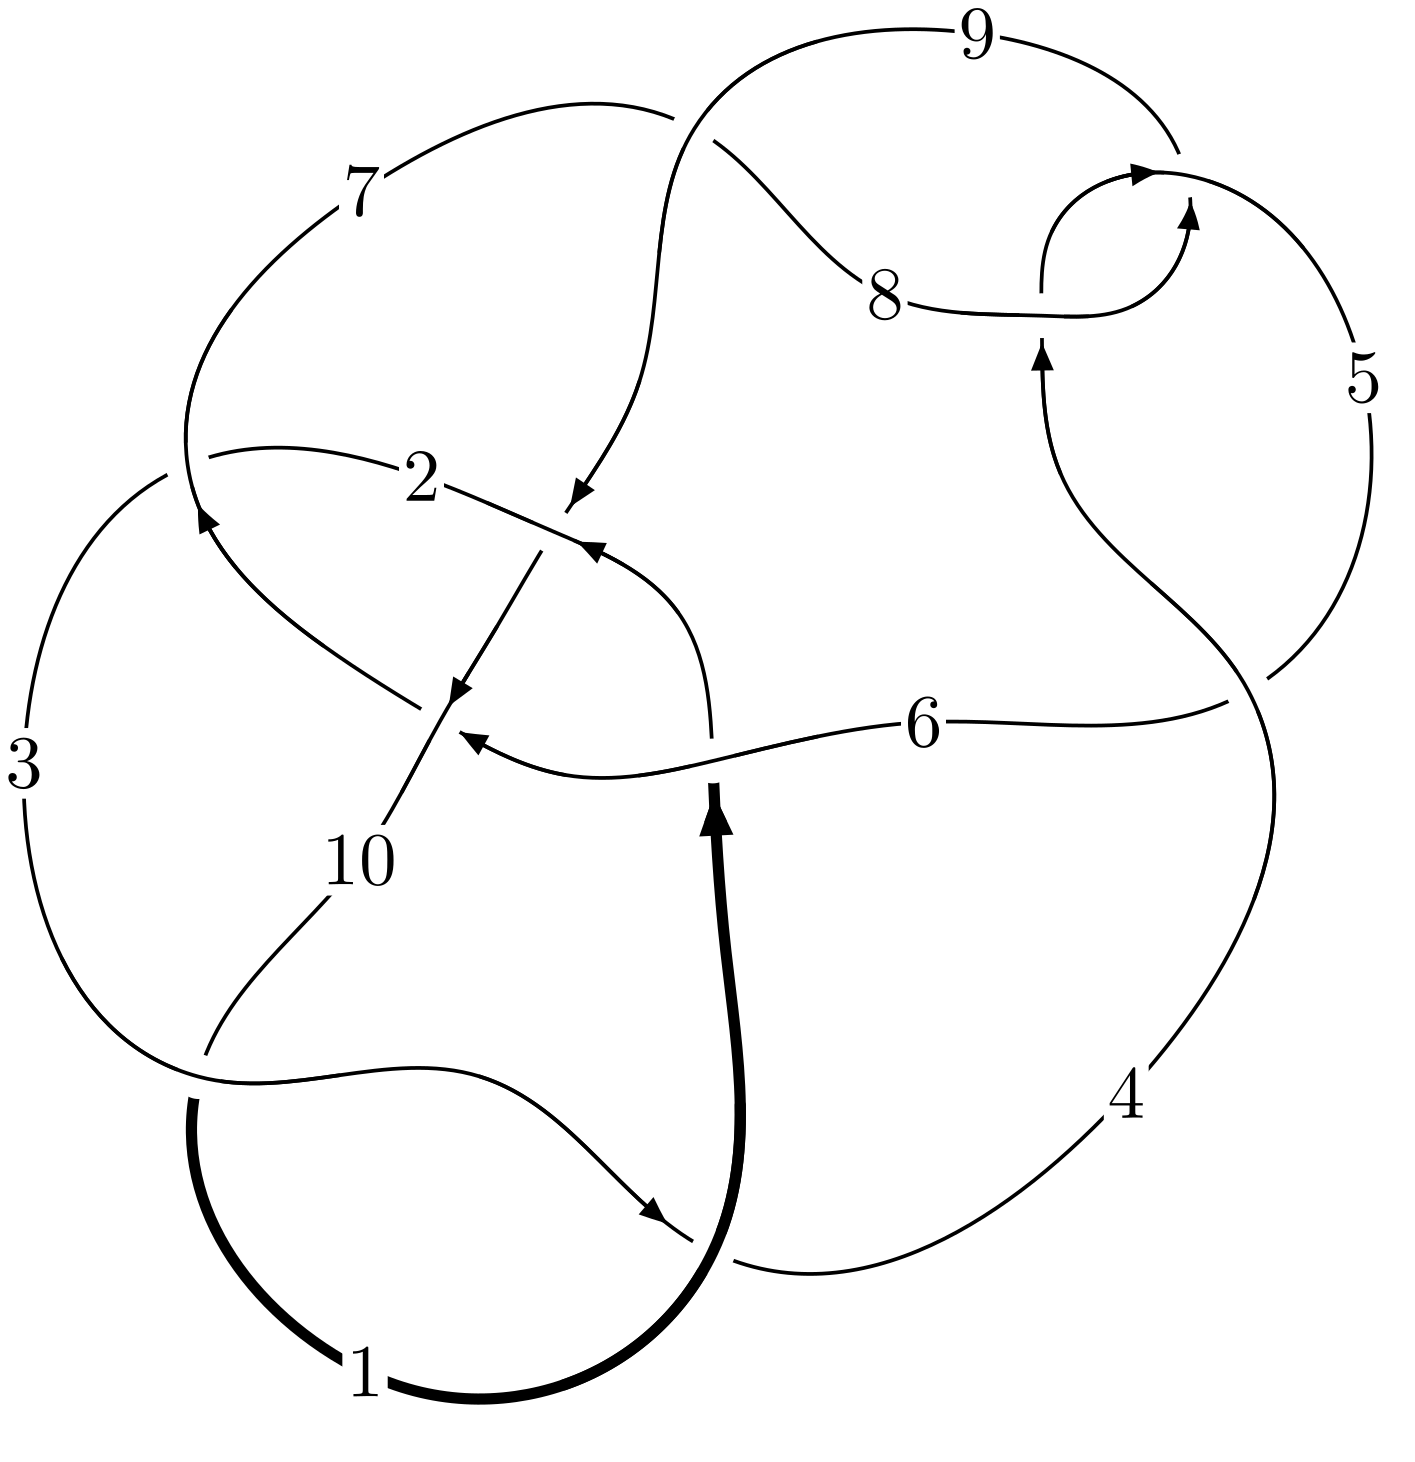
\includegraphics[width=112pt]{../../../GIT/diagram.site/Diagrams/png/171_10_87.png}\\
\ \ \ A knot diagram\footnotemark}&
\allowdisplaybreaks
\textbf{Linearized knot diagam} \\
\cline{2-2}
 &
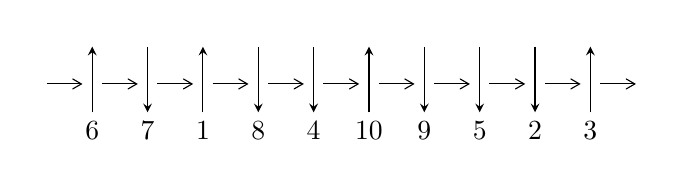
\begin{tikzpicture}[x=20pt, y=17pt]
	% nodes
	\node (C0) at (0, 0) {};
	\node (C1) at (1, 0) {};
	\node (C1U) at (1, +1) {};
	\node (C1D) at (1, -1) {6};

	\node (C2) at (2, 0) {};
	\node (C2U) at (2, +1) {};
	\node (C2D) at (2, -1) {7};

	\node (C3) at (3, 0) {};
	\node (C3U) at (3, +1) {};
	\node (C3D) at (3, -1) {1};

	\node (C4) at (4, 0) {};
	\node (C4U) at (4, +1) {};
	\node (C4D) at (4, -1) {8};

	\node (C5) at (5, 0) {};
	\node (C5U) at (5, +1) {};
	\node (C5D) at (5, -1) {4};

	\node (C6) at (6, 0) {};
	\node (C6U) at (6, +1) {};
	\node (C6D) at (6, -1) {10};

	\node (C7) at (7, 0) {};
	\node (C7U) at (7, +1) {};
	\node (C7D) at (7, -1) {9};

	\node (C8) at (8, 0) {};
	\node (C8U) at (8, +1) {};
	\node (C8D) at (8, -1) {5};

	\node (C9) at (9, 0) {};
	\node (C9U) at (9, +1) {};
	\node (C9D) at (9, -1) {2};

	\node (C10) at (10, 0) {};
	\node (C10U) at (10, +1) {};
	\node (C10D) at (10, -1) {3};
	\node (C11) at (11, 0) {};

	% arrows
	\draw[->,>={angle 60}]
	(C0) edge (C1) (C1) edge (C2) (C2) edge (C3) (C3) edge (C4) (C4) edge (C5) (C5) edge (C6) (C6) edge (C7) (C7) edge (C8) (C8) edge (C9) (C9) edge (C10) (C10) edge (C11) ;	\draw[->,>=stealth]
	(C1D) edge (C1U) (C2U) edge (C2D) (C3D) edge (C3U) (C4U) edge (C4D) (C5U) edge (C5D) (C6D) edge (C6U) (C7U) edge (C7D) (C8U) edge (C8D) (C9U) edge (C9D) (C10D) edge (C10U) ;
	\end{tikzpicture} \\
\hhline{~~} \\& 
\textbf{Solving Sequence} \\ \cline{2-2} 
 &
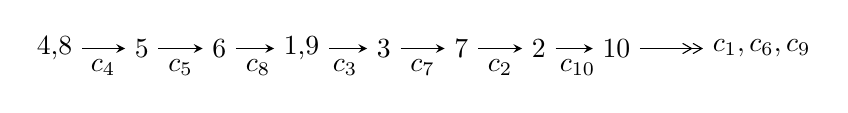
\begin{tikzpicture}[x=28pt, y=7pt]
	% node
	\node (A0) at (-1/8, 0) {4,8};
	\node (A1) at (1, 0) {5};
	\node (A2) at (2, 0) {6};
	\node (A3) at (49/16, 0) {1,9};
	\node (A4) at (33/8, 0) {3};
	\node (A5) at (41/8, 0) {7};
	\node (A6) at (49/8, 0) {2};
	\node (A7) at (57/8, 0) {10};
	\node (C1) at (1/2, -1) {$c_{4}$};
	\node (C2) at (3/2, -1) {$c_{5}$};
	\node (C3) at (5/2, -1) {$c_{8}$};
	\node (C4) at (29/8, -1) {$c_{3}$};
	\node (C5) at (37/8, -1) {$c_{7}$};
	\node (C6) at (45/8, -1) {$c_{2}$};
	\node (C7) at (53/8, -1) {$c_{10}$};
	\node (A8) at (9, 0) {$c_{1},c_{6},c_{9}$};

	% edge
	\draw[->,>=stealth]	
	(A0) edge (A1) (A1) edge (A2) (A2) edge (A3) (A3) edge (A4) (A4) edge (A5) (A5) edge (A6) (A6) edge (A7) ;
	\draw[->>,>={angle 60}]	
	(A7) edge (A8);
\end{tikzpicture} \\ 

\end{tabular} \\

\footnotetext{
The image of knot diagram is generated by the software ``\textbf{Draw programme}" developed by Andrew Bartholomew(\url{http://www.layer8.co.uk/maths/draw/index.htm\#Running-draw}), where we modified some parts for our purpose(\url{https://github.com/CATsTAILs/LinksPainter}).
}\phantom \\ \newline 
\centering \textbf{Ideals for irreducible components\footnotemark of $X_{\text{par}}$} 
 
\begin{align*}
I^u_{1}&=\langle 
2225248116121 u^{40}-2393989479567 u^{39}+\cdots+10297376929134 b-6012630756121,\\
\phantom{I^u_{1}}&\phantom{= \langle  }-31071718506119 u^{40}+39367206545589 u^{39}+\cdots+5148688464567 a-44602733573152,\\
\phantom{I^u_{1}}&\phantom{= \langle  }u^{41}-2 u^{40}+\cdots- u-1\rangle \\
I^u_{2}&=\langle 
b-1,\;a-1,\;u-1\rangle \\
\\
\end{align*}
\raggedright * 2 irreducible components of $\dim_{\mathbb{C}}=0$, with total 42 representations.\\
\footnotetext{All coefficients of polynomials are rational numbers. But the coefficients are sometimes approximated in decimal forms when there is not enough margin.}
\newpage
\renewcommand{\arraystretch}{1}
\centering \section*{I. $I^u_{1}= \langle 2.23\times10^{12} u^{40}-2.39\times10^{12} u^{39}+\cdots+1.03\times10^{13} b-6.01\times10^{12},\;-3.11\times10^{13} u^{40}+3.94\times10^{13} u^{39}+\cdots+5.15\times10^{12} a-4.46\times10^{13},\;u^{41}-2 u^{40}+\cdots- u-1 \rangle$}
\flushleft \textbf{(i) Arc colorings}\\
\begin{tabular}{m{7pt} m{180pt} m{7pt} m{180pt} }
\flushright $a_{4}=$&$\begin{pmatrix}1\\0\end{pmatrix}$ \\
\flushright $a_{8}=$&$\begin{pmatrix}0\\u\end{pmatrix}$ \\
\flushright $a_{5}=$&$\begin{pmatrix}1\\u^2\end{pmatrix}$ \\
\flushright $a_{6}=$&$\begin{pmatrix}- u^2+1\\u^2\end{pmatrix}$ \\
\flushright $a_{1}=$&$\begin{pmatrix}6.03488 u^{40}-7.64606 u^{39}+\cdots+20.1260 u+8.66293\\-0.216099 u^{40}+0.232485 u^{39}+\cdots-1.20415 u+0.583899\end{pmatrix}$ \\
\flushright $a_{9}=$&$\begin{pmatrix}- u\\- u^3+u\end{pmatrix}$ \\
\flushright $a_{3}=$&$\begin{pmatrix}5.64438 u^{40}-7.18325 u^{39}+\cdots+18.2918 u+8.93217\\-0.135606 u^{40}+0.0700585 u^{39}+\cdots-1.18339 u+0.664403\end{pmatrix}$ \\
\flushright $a_{7}=$&$\begin{pmatrix}u^3\\u^5- u^3+u\end{pmatrix}$ \\
\flushright $a_{2}=$&$\begin{pmatrix}4.44062 u^{40}-5.31684 u^{39}+\cdots+13.7767 u+7.07457\\-1.46774 u^{40}+1.54335 u^{39}+\cdots-6.10178 u-1.46782\end{pmatrix}$ \\
\flushright $a_{10}=$&$\begin{pmatrix}1.00290 u^{40}-1.84189 u^{39}+\cdots+5.12751 u+1.12239\\-0.839015 u^{40}+1.67515 u^{39}+\cdots-0.958478 u-0.838993\end{pmatrix}$\\&\end{tabular}
\flushleft \textbf{(ii) Obstruction class $= -1$}\\~\\
\flushleft \textbf{(iii) Cusp Shapes $= \frac{23238917313784}{1716229488189} u^{40}-\frac{10481023528134}{572076496063} u^{39}+\cdots+\frac{28692506559598}{572076496063} u+\frac{39302820789020}{1716229488189}$}\\~\\
\newpage\renewcommand{\arraystretch}{1}
\flushleft \textbf{(iv) u-Polynomials at the component}\newline \\
\begin{tabular}{m{50pt}|m{274pt}}
Crossings & \hspace{64pt}u-Polynomials at each crossing \\
\hline $$\begin{aligned}c_{1}\end{aligned}$$&$\begin{aligned}
&u^{41}+8 u^{39}+\cdots+687 u+229
\end{aligned}$\\
\hline $$\begin{aligned}c_{2}\end{aligned}$$&$\begin{aligned}
&u^{41}+2 u^{40}+\cdots-97 u+29
\end{aligned}$\\
\hline $$\begin{aligned}c_{3},c_{10}\end{aligned}$$&$\begin{aligned}
&u^{41}+2 u^{40}+\cdots+9 u+1
\end{aligned}$\\
\hline $$\begin{aligned}c_{4},c_{8}\end{aligned}$$&$\begin{aligned}
&u^{41}+2 u^{40}+\cdots- u+1
\end{aligned}$\\
\hline $$\begin{aligned}c_{5},c_{7}\end{aligned}$$&$\begin{aligned}
&u^{41}+12 u^{40}+\cdots+5 u+1
\end{aligned}$\\
\hline $$\begin{aligned}c_{6}\end{aligned}$$&$\begin{aligned}
&u^{41}+4 u^{40}+\cdots+u+1
\end{aligned}$\\
\hline $$\begin{aligned}c_{9}\end{aligned}$$&$\begin{aligned}
&u^{41}-7 u^{40}+\cdots+6 u-2
\end{aligned}$\\
\hline
\end{tabular}\\~\\
\newpage\renewcommand{\arraystretch}{1}
\flushleft \textbf{(v) Riley Polynomials at the component}\newline \\
\begin{tabular}{m{50pt}|m{274pt}}
Crossings & \hspace{64pt}Riley Polynomials at each crossing \\
\hline $$\begin{aligned}c_{1}\end{aligned}$$&$\begin{aligned}
&y^{41}+16 y^{40}+\cdots+1271637 y-52441
\end{aligned}$\\
\hline $$\begin{aligned}c_{2}\end{aligned}$$&$\begin{aligned}
&y^{41}+48 y^{40}+\cdots-7063 y-841
\end{aligned}$\\
\hline $$\begin{aligned}c_{3},c_{10}\end{aligned}$$&$\begin{aligned}
&y^{41}-32 y^{40}+\cdots+141 y-1
\end{aligned}$\\
\hline $$\begin{aligned}c_{4},c_{8}\end{aligned}$$&$\begin{aligned}
&y^{41}-12 y^{40}+\cdots+5 y-1
\end{aligned}$\\
\hline $$\begin{aligned}c_{5},c_{7}\end{aligned}$$&$\begin{aligned}
&y^{41}+36 y^{40}+\cdots+5 y-1
\end{aligned}$\\
\hline $$\begin{aligned}c_{6}\end{aligned}$$&$\begin{aligned}
&y^{41}-8 y^{40}+\cdots+5 y-1
\end{aligned}$\\
\hline $$\begin{aligned}c_{9}\end{aligned}$$&$\begin{aligned}
&y^{41}+9 y^{40}+\cdots-16 y-4
\end{aligned}$\\
\hline
\end{tabular}\\~\\
\newpage\flushleft \textbf{(vi) Complex Volumes and Cusp Shapes}
$$\begin{array}{c|c|c}  
\text{Solutions to }I^u_{1}& \I (\text{vol} + \sqrt{-1}CS) & \text{Cusp shape}\\
 \hline 
\begin{aligned}
u &= \phantom{-}0.903206 + 0.396002 I \\
a &= \phantom{-}1.211920 + 0.667053 I \\
b &= -0.408078 + 0.420450 I\end{aligned}
 & -1.94008 - 1.34771 I & -7.61480 + 3.42502 I \\ \hline\begin{aligned}
u &= \phantom{-}0.903206 - 0.396002 I \\
a &= \phantom{-}1.211920 - 0.667053 I \\
b &= -0.408078 - 0.420450 I\end{aligned}
 & -1.94008 + 1.34771 I & -7.61480 - 3.42502 I \\ \hline\begin{aligned}
u &= -0.952455 + 0.222261 I \\
a &= -0.211328 + 0.932061 I \\
b &= -0.096162 + 0.914015 I\end{aligned}
 & -2.78156 + 3.84619 I & -6.97849 - 6.75687 I \\ \hline\begin{aligned}
u &= -0.952455 - 0.222261 I \\
a &= -0.211328 - 0.932061 I \\
b &= -0.096162 - 0.914015 I\end{aligned}
 & -2.78156 - 3.84619 I & -6.97849 + 6.75687 I \\ \hline\begin{aligned}
u &= -0.821825 + 0.760247 I \\
a &= \phantom{-}0.450451 - 0.306050 I \\
b &= \phantom{-}0.335334 - 0.324976 I\end{aligned}
 & \phantom{-}3.49362 + 1.78935 I & \phantom{-}0.87448 - 4.34492 I \\ \hline\begin{aligned}
u &= -0.821825 - 0.760247 I \\
a &= \phantom{-}0.450451 + 0.306050 I \\
b &= \phantom{-}0.335334 + 0.324976 I\end{aligned}
 & \phantom{-}3.49362 - 1.78935 I & \phantom{-}0.87448 + 4.34492 I \\ \hline\begin{aligned}
u &= \phantom{-}0.866850\phantom{ +0.000000I} \\
a &= \phantom{-}0.639506\phantom{ +0.000000I} \\
b &= -0.0835204\phantom{ +0.000000I}\end{aligned}
 & -1.43130\phantom{ +0.000000I} & -6.87200\phantom{ +0.000000I} \\ \hline\begin{aligned}
u &= \phantom{-}0.798878 + 0.810698 I \\
a &= \phantom{-}0.377223 - 0.719870 I \\
b &= \phantom{-}0.265202 + 1.192170 I\end{aligned}
 & \phantom{-}3.76974 + 2.25598 I & \phantom{-}1.50138 - 3.41744 I \\ \hline\begin{aligned}
u &= \phantom{-}0.798878 - 0.810698 I \\
a &= \phantom{-}0.377223 + 0.719870 I \\
b &= \phantom{-}0.265202 - 1.192170 I\end{aligned}
 & \phantom{-}3.76974 - 2.25598 I & \phantom{-}1.50138 + 3.41744 I \\ \hline\begin{aligned}
u &= -1.102330 + 0.334587 I \\
a &= \phantom{-}0.338270 - 1.284530 I \\
b &= -1.253450 - 0.430907 I\end{aligned}
 & \phantom{-}0.85372 + 8.63849 I & -1.84811 - 8.19635 I\\
 \hline 
 \end{array}$$\newpage$$\begin{array}{c|c|c}  
\text{Solutions to }I^u_{1}& \I (\text{vol} + \sqrt{-1}CS) & \text{Cusp shape}\\
 \hline 
\begin{aligned}
u &= -1.102330 - 0.334587 I \\
a &= \phantom{-}0.338270 + 1.284530 I \\
b &= -1.253450 + 0.430907 I\end{aligned}
 & \phantom{-}0.85372 - 8.63849 I & -1.84811 + 8.19635 I \\ \hline\begin{aligned}
u &= -0.058442 + 0.843545 I \\
a &= \phantom{-}1.57943 - 0.15589 I \\
b &= -1.284700 + 0.271028 I\end{aligned}
 & \phantom{-}4.36449 - 4.62926 I & \phantom{-}4.68493 + 4.91932 I \\ \hline\begin{aligned}
u &= -0.058442 - 0.843545 I \\
a &= \phantom{-}1.57943 + 0.15589 I \\
b &= -1.284700 - 0.271028 I\end{aligned}
 & \phantom{-}4.36449 + 4.62926 I & \phantom{-}4.68493 - 4.91932 I \\ \hline\begin{aligned}
u &= -0.883648 + 0.770325 I \\
a &= -3.62989 + 1.11022 I \\
b &= \phantom{-}1.134150 + 0.025263 I\end{aligned}
 & \phantom{-}5.18095 + 2.90757 I & -15.8800 + 0. I\phantom{ +0.000000I} \\ \hline\begin{aligned}
u &= -0.883648 - 0.770325 I \\
a &= -3.62989 - 1.11022 I \\
b &= \phantom{-}1.134150 - 0.025263 I\end{aligned}
 & \phantom{-}5.18095 - 2.90757 I & -15.8800 + 0. I\phantom{ +0.000000I} \\ \hline\begin{aligned}
u &= \phantom{-}0.760286 + 0.907829 I \\
a &= \phantom{-}1.73221 + 0.34788 I \\
b &= -1.45266 - 0.46932 I\end{aligned}
 & \phantom{-}9.17940 + 7.97252 I & \phantom{-}3.27060 - 3.71618 I \\ \hline\begin{aligned}
u &= \phantom{-}0.760286 - 0.907829 I \\
a &= \phantom{-}1.73221 - 0.34788 I \\
b &= -1.45266 + 0.46932 I\end{aligned}
 & \phantom{-}9.17940 - 7.97252 I & \phantom{-}3.27060 + 3.71618 I \\ \hline\begin{aligned}
u &= \phantom{-}0.866672 + 0.809557 I \\
a &= -1.56395 - 1.02120 I \\
b &= \phantom{-}1.60494 + 0.57469 I\end{aligned}
 & \phantom{-}7.77351 - 0.87153 I & \phantom{-}6.95024 - 0.30904 I \\ \hline\begin{aligned}
u &= \phantom{-}0.866672 - 0.809557 I \\
a &= -1.56395 + 1.02120 I \\
b &= \phantom{-}1.60494 - 0.57469 I\end{aligned}
 & \phantom{-}7.77351 + 0.87153 I & \phantom{-}6.95024 + 0.30904 I \\ \hline\begin{aligned}
u &= -0.929908 + 0.739442 I \\
a &= \phantom{-}0.037024 + 0.508793 I \\
b &= \phantom{-}0.197100 + 0.379729 I\end{aligned}
 & \phantom{-}3.15987 + 3.90045 I & -0.31532 - 1.57295 I\\
 \hline 
 \end{array}$$\newpage$$\begin{array}{c|c|c}  
\text{Solutions to }I^u_{1}& \I (\text{vol} + \sqrt{-1}CS) & \text{Cusp shape}\\
 \hline 
\begin{aligned}
u &= -0.929908 - 0.739442 I \\
a &= \phantom{-}0.037024 - 0.508793 I \\
b &= \phantom{-}0.197100 - 0.379729 I\end{aligned}
 & \phantom{-}3.15987 - 3.90045 I & -0.31532 + 1.57295 I \\ \hline\begin{aligned}
u &= -0.744475 + 0.942248 I \\
a &= \phantom{-}1.62214 - 0.18187 I \\
b &= -1.310630 + 0.070763 I\end{aligned}
 & \phantom{-}8.52020 + 0.56768 I & \phantom{-}6.81847 - 0.32338 I \\ \hline\begin{aligned}
u &= -0.744475 - 0.942248 I \\
a &= \phantom{-}1.62214 + 0.18187 I \\
b &= -1.310630 - 0.070763 I\end{aligned}
 & \phantom{-}8.52020 - 0.56768 I & \phantom{-}6.81847 + 0.32338 I \\ \hline\begin{aligned}
u &= -0.739440 + 0.286658 I \\
a &= \phantom{-}0.11659 + 1.68574 I \\
b &= \phantom{-}1.073000 + 0.545709 I\end{aligned}
 & \phantom{-}1.56831 + 2.54987 I & \phantom{-}1.57226 - 7.77175 I \\ \hline\begin{aligned}
u &= -0.739440 - 0.286658 I \\
a &= \phantom{-}0.11659 - 1.68574 I \\
b &= \phantom{-}1.073000 - 0.545709 I\end{aligned}
 & \phantom{-}1.56831 - 2.54987 I & \phantom{-}1.57226 + 7.77175 I \\ \hline\begin{aligned}
u &= \phantom{-}0.913744 + 0.795988 I \\
a &= -2.19807 - 1.07996 I \\
b &= \phantom{-}1.55855 - 0.65970 I\end{aligned}
 & \phantom{-}7.62795 - 5.14257 I & \phantom{-}6.43416 + 5.95767 I \\ \hline\begin{aligned}
u &= \phantom{-}0.913744 - 0.795988 I \\
a &= -2.19807 + 1.07996 I \\
b &= \phantom{-}1.55855 + 0.65970 I\end{aligned}
 & \phantom{-}7.62795 + 5.14257 I & \phantom{-}6.43416 - 5.95767 I \\ \hline\begin{aligned}
u &= \phantom{-}1.191150 + 0.227807 I \\
a &= -0.076211 + 0.412771 I \\
b &= -1.116560 - 0.153454 I\end{aligned}
 & \phantom{-}0.067811 + 0.953358 I & \phantom{-}2.02910 - 7.42558 I \\ \hline\begin{aligned}
u &= \phantom{-}1.191150 - 0.227807 I \\
a &= -0.076211 - 0.412771 I \\
b &= -1.116560 + 0.153454 I\end{aligned}
 & \phantom{-}0.067811 - 0.953358 I & \phantom{-}2.02910 + 7.42558 I \\ \hline\begin{aligned}
u &= \phantom{-}0.960612 + 0.767884 I \\
a &= -1.113770 + 0.253317 I \\
b &= \phantom{-}0.163245 - 1.244780 I\end{aligned}
 & \phantom{-}3.27367 - 8.18385 I & \phantom{-0.000000 -}0. + 8.35233 I\\
 \hline 
 \end{array}$$\newpage$$\begin{array}{c|c|c}  
\text{Solutions to }I^u_{1}& \I (\text{vol} + \sqrt{-1}CS) & \text{Cusp shape}\\
 \hline 
\begin{aligned}
u &= \phantom{-}0.960612 - 0.767884 I \\
a &= -1.113770 - 0.253317 I \\
b &= \phantom{-}0.163245 + 1.244780 I\end{aligned}
 & \phantom{-}3.27367 + 8.18385 I & \phantom{-0.000000 } 0. - 8.35233 I \\ \hline\begin{aligned}
u &= \phantom{-}0.748657 + 0.093307 I \\
a &= \phantom{-}0.47886 - 4.75552 I \\
b &= \phantom{-}0.938830 - 0.044980 I\end{aligned}
 & \phantom{-}0.431185 - 0.284475 I & \phantom{-}13.1815 - 15.1990 I \\ \hline\begin{aligned}
u &= \phantom{-}0.748657 - 0.093307 I \\
a &= \phantom{-}0.47886 + 4.75552 I \\
b &= \phantom{-}0.938830 + 0.044980 I\end{aligned}
 & \phantom{-}0.431185 + 0.284475 I & \phantom{-}13.1815 + 15.1990 I \\ \hline\begin{aligned}
u &= \phantom{-}1.022750 + 0.797628 I \\
a &= \phantom{-}1.90383 + 1.42431 I \\
b &= -1.44670 + 0.51890 I\end{aligned}
 & \phantom{-}8.3544 - 14.2736 I & \phantom{-0.000000 -}0. + 8.33140 I \\ \hline\begin{aligned}
u &= \phantom{-}1.022750 - 0.797628 I \\
a &= \phantom{-}1.90383 - 1.42431 I \\
b &= -1.44670 - 0.51890 I\end{aligned}
 & \phantom{-}8.3544 + 14.2736 I & \phantom{-0.000000 } 0. - 8.33140 I \\ \hline\begin{aligned}
u &= -1.045230 + 0.812235 I \\
a &= \phantom{-}1.41367 - 1.18781 I \\
b &= -1.277530 - 0.155370 I\end{aligned}
 & \phantom{-}7.57848 + 5.87702 I & \phantom{-0.000000 } 0. - 5.65225 I \\ \hline\begin{aligned}
u &= -1.045230 - 0.812235 I \\
a &= \phantom{-}1.41367 + 1.18781 I \\
b &= -1.277530 + 0.155370 I\end{aligned}
 & \phantom{-}7.57848 - 5.87702 I & \phantom{-0.000000 -}0. + 5.65225 I \\ \hline\begin{aligned}
u &= \phantom{-}0.039502 + 0.458105 I \\
a &= \phantom{-}0.880104 + 0.384951 I \\
b &= \phantom{-}0.142705 - 0.550416 I\end{aligned}
 & \phantom{-}0.05414 - 1.50218 I & \phantom{-}0.18723 + 4.24532 I \\ \hline\begin{aligned}
u &= \phantom{-}0.039502 - 0.458105 I \\
a &= \phantom{-}0.880104 - 0.384951 I \\
b &= \phantom{-}0.142705 + 0.550416 I\end{aligned}
 & \phantom{-}0.05414 + 1.50218 I & \phantom{-}0.18723 - 4.24532 I \\ \hline\begin{aligned}
u &= -0.361128 + 0.264161 I \\
a &= -0.168271 + 0.663616 I \\
b &= \phantom{-}1.275180 - 0.127224 I\end{aligned}
 & \phantom{-}2.56290 - 0.10225 I & \phantom{-}4.38337 - 2.22967 I\\
 \hline 
 \end{array}$$\newpage$$\begin{array}{c|c|c}  
\text{Solutions to }I^u_{1}& \I (\text{vol} + \sqrt{-1}CS) & \text{Cusp shape}\\
 \hline 
\begin{aligned}
u &= -0.361128 - 0.264161 I \\
a &= -0.168271 - 0.663616 I \\
b &= \phantom{-}1.275180 + 0.127224 I\end{aligned}
 & \phantom{-}2.56290 + 0.10225 I & \phantom{-}4.38337 + 2.22967 I\\
 \hline 
 \end{array}$$\newpage\newpage\renewcommand{\arraystretch}{1}
\centering \section*{II. $I^u_{2}= \langle b-1,\;a-1,\;u-1 \rangle$}
\flushleft \textbf{(i) Arc colorings}\\
\begin{tabular}{m{7pt} m{180pt} m{7pt} m{180pt} }
\flushright $a_{4}=$&$\begin{pmatrix}1\\0\end{pmatrix}$ \\
\flushright $a_{8}=$&$\begin{pmatrix}0\\1\end{pmatrix}$ \\
\flushright $a_{5}=$&$\begin{pmatrix}1\\1\end{pmatrix}$ \\
\flushright $a_{6}=$&$\begin{pmatrix}0\\1\end{pmatrix}$ \\
\flushright $a_{1}=$&$\begin{pmatrix}1\\1\end{pmatrix}$ \\
\flushright $a_{9}=$&$\begin{pmatrix}-1\\0\end{pmatrix}$ \\
\flushright $a_{3}=$&$\begin{pmatrix}2\\1\end{pmatrix}$ \\
\flushright $a_{7}=$&$\begin{pmatrix}1\\1\end{pmatrix}$ \\
\flushright $a_{2}=$&$\begin{pmatrix}1\\0\end{pmatrix}$ \\
\flushright $a_{10}=$&$\begin{pmatrix}-1\\0\end{pmatrix}$\\&\end{tabular}
\flushleft \textbf{(ii) Obstruction class $= 1$}\\~\\
\flushleft \textbf{(iii) Cusp Shapes $= 0$}\\~\\
\newpage\renewcommand{\arraystretch}{1}
\flushleft \textbf{(iv) u-Polynomials at the component}\newline \\
\begin{tabular}{m{50pt}|m{274pt}}
Crossings & \hspace{64pt}u-Polynomials at each crossing \\
\hline $$\begin{aligned}c_{1},c_{2},c_{3}\\c_{4},c_{6},c_{7}\end{aligned}$$&$\begin{aligned}
&u-1
\end{aligned}$\\
\hline $$\begin{aligned}c_{5},c_{8},c_{10}\end{aligned}$$&$\begin{aligned}
&u+1
\end{aligned}$\\
\hline $$\begin{aligned}c_{9}\end{aligned}$$&$\begin{aligned}
&u
\end{aligned}$\\
\hline
\end{tabular}\\~\\
\newpage\renewcommand{\arraystretch}{1}
\flushleft \textbf{(v) Riley Polynomials at the component}\newline \\
\begin{tabular}{m{50pt}|m{274pt}}
Crossings & \hspace{64pt}Riley Polynomials at each crossing \\
\hline $$\begin{aligned}c_{1},c_{2},c_{3}\\c_{4},c_{5},c_{6}\\c_{7},c_{8},c_{10}\end{aligned}$$&$\begin{aligned}
&y-1
\end{aligned}$\\
\hline $$\begin{aligned}c_{9}\end{aligned}$$&$\begin{aligned}
&y
\end{aligned}$\\
\hline
\end{tabular}\\~\\
\newpage\flushleft \textbf{(vi) Complex Volumes and Cusp Shapes}
$$\begin{array}{c|c|c}  
\text{Solutions to }I^u_{2}& \I (\text{vol} + \sqrt{-1}CS) & \text{Cusp shape}\\
 \hline 
\begin{aligned}
u &= \phantom{-}1.00000\phantom{ +0.000000I} \\
a &= \phantom{-}1.00000\phantom{ +0.000000I} \\
b &= \phantom{-}1.00000\phantom{ +0.000000I}\end{aligned}
 & \phantom{-0.000000 } 0 & \phantom{-0.000000 } 0\\
 \hline 
 \end{array}$$\newpage
\newpage\renewcommand{\arraystretch}{1}
\centering \section*{ III. u-Polynomials}
\begin{tabular}{m{50pt}|m{274pt}}
Crossings & \hspace{64pt}u-Polynomials at each crossing \\
\hline $$\begin{aligned}c_{1}\end{aligned}$$&$\begin{aligned}
&(u-1)(u^{41}+8 u^{39}+\cdots+687 u+229)
\end{aligned}$\\
\hline $$\begin{aligned}c_{2}\end{aligned}$$&$\begin{aligned}
&(u-1)(u^{41}+2 u^{40}+\cdots-97 u+29)
\end{aligned}$\\
\hline $$\begin{aligned}c_{3}\end{aligned}$$&$\begin{aligned}
&(u-1)(u^{41}+2 u^{40}+\cdots+9 u+1)
\end{aligned}$\\
\hline $$\begin{aligned}c_{4}\end{aligned}$$&$\begin{aligned}
&(u-1)(u^{41}+2 u^{40}+\cdots- u+1)
\end{aligned}$\\
\hline $$\begin{aligned}c_{5}\end{aligned}$$&$\begin{aligned}
&(u+1)(u^{41}+12 u^{40}+\cdots+5 u+1)
\end{aligned}$\\
\hline $$\begin{aligned}c_{6}\end{aligned}$$&$\begin{aligned}
&(u-1)(u^{41}+4 u^{40}+\cdots+u+1)
\end{aligned}$\\
\hline $$\begin{aligned}c_{7}\end{aligned}$$&$\begin{aligned}
&(u-1)(u^{41}+12 u^{40}+\cdots+5 u+1)
\end{aligned}$\\
\hline $$\begin{aligned}c_{8}\end{aligned}$$&$\begin{aligned}
&(u+1)(u^{41}+2 u^{40}+\cdots- u+1)
\end{aligned}$\\
\hline $$\begin{aligned}c_{9}\end{aligned}$$&$\begin{aligned}
&u(u^{41}-7 u^{40}+\cdots+6 u-2)
\end{aligned}$\\
\hline $$\begin{aligned}c_{10}\end{aligned}$$&$\begin{aligned}
&(u+1)(u^{41}+2 u^{40}+\cdots+9 u+1)
\end{aligned}$\\
\hline
\end{tabular}\newpage\renewcommand{\arraystretch}{1}
\centering \section*{ IV. Riley Polynomials}
\begin{tabular}{m{50pt}|m{274pt}}
Crossings & \hspace{64pt}Riley Polynomials at each crossing \\
\hline $$\begin{aligned}c_{1}\end{aligned}$$&$\begin{aligned}
&(y-1)(y^{41}+16 y^{40}+\cdots+1271637 y-52441)
\end{aligned}$\\
\hline $$\begin{aligned}c_{2}\end{aligned}$$&$\begin{aligned}
&(y-1)(y^{41}+48 y^{40}+\cdots-7063 y-841)
\end{aligned}$\\
\hline $$\begin{aligned}c_{3},c_{10}\end{aligned}$$&$\begin{aligned}
&(y-1)(y^{41}-32 y^{40}+\cdots+141 y-1)
\end{aligned}$\\
\hline $$\begin{aligned}c_{4},c_{8}\end{aligned}$$&$\begin{aligned}
&(y-1)(y^{41}-12 y^{40}+\cdots+5 y-1)
\end{aligned}$\\
\hline $$\begin{aligned}c_{5},c_{7}\end{aligned}$$&$\begin{aligned}
&(y-1)(y^{41}+36 y^{40}+\cdots+5 y-1)
\end{aligned}$\\
\hline $$\begin{aligned}c_{6}\end{aligned}$$&$\begin{aligned}
&(y-1)(y^{41}-8 y^{40}+\cdots+5 y-1)
\end{aligned}$\\
\hline $$\begin{aligned}c_{9}\end{aligned}$$&$\begin{aligned}
&y(y^{41}+9 y^{40}+\cdots-16 y-4)
\end{aligned}$\\
\hline
\end{tabular}
\vskip 2pc
\end{document}